% 03_results_existing.tex
% Results subsections whose numbers already exist in macros.tex (pass 1).
% Pass 2 fills the marked holes once the J10/J11/J12 numbers are macros.
% Every number in prose is a \fs... macro; \fsTODO marks a number that does
% not exist yet. Vocabulary follows REVISION_FACTS.md section 3.

\section{Results}
\label{sec:results}

% PASS2: 3.1 accuracy and calibration goes here (tab:accuracy, fig:calibration)

\subsection{Committee disagreement identifies high-error structures at fixed system size}
\label{sec:fixedsize}

This subsection asks the first of the two questions set out in the Introduction:
does the exact committee statistic identify the structures on which the
committee-mean forces are most wrong? We call this property error-ranking
quality. Nothing is fitted in the analysis, so there is no risk of leakage and
the full evaluation set of each system is used.

Six molecular systems are compared, each with a fixed number of atoms. Three are
the 3BPA molecule~\citep{kovacs2021beyond} at 1200\,K, scored by shared-trunk
committees that were trained at 300\,K and built in three ways: disjoint heads,
overlapping heads, and identical data (Methods). The other three are ethanol,
aspirin and azobenzene from rMD17~\citep{christensen2020role}, scored by one
committee with disjoint heads that was trained jointly on all ten rMD17
molecules. The error target is the largest per-atom force error in a structure,
$e_{\max}$, and the positives are the top 5\% of structures by that target. The
ranking metric is the area under the receiver operating characteristic curve
(AUROC): the probability that a randomly chosen positive structure is ranked
above a randomly chosen other structure, so that chance is one half and a
perfect ranking is one. Intervals are paired moving-block
bootstraps~\citep{kunsch1989jackknife} with the block length set by the measured
autocorrelation time of each error series.

Three structure-level scores are formed from the per-coordinate head variance
$v_d$ (Methods). The global score is the sum of $v_d$ over all $3N$ coordinates.
The max-component score is the largest $\sqrt{v_d}$ over coordinates, and is
the rule used by \citet{beck2025committee}. The max-atom score is the largest
per-atom standard deviation. The global score ranks the top-5\% highest-error
structures at AUROC $\fsFactorALo$--$\fsFactorAHi$ across the six systems, with
the random null at chance (Figure~\ref{fig:factora}). The committee is therefore
informative but far from perfect. The per-atom and reliability views of the same
committees are in Table~\ref{tab:accuracy} and Figure~\ref{fig:calibration}.

\begin{figure}[t]
\centering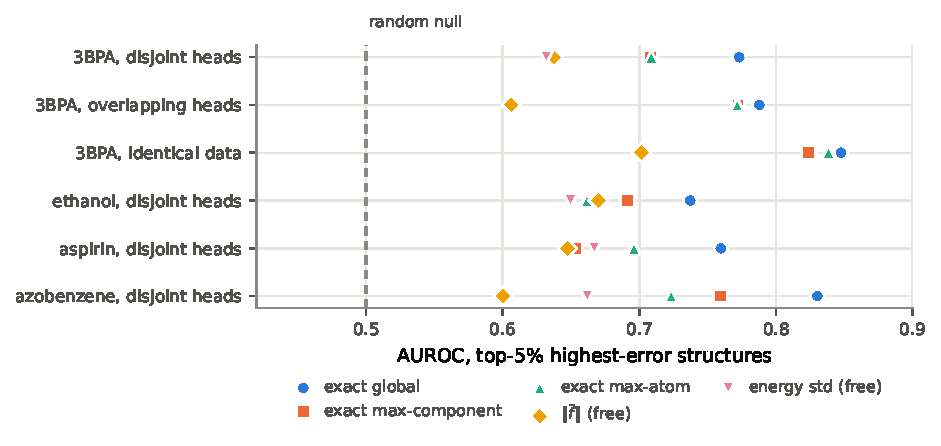
\includegraphics[width=\linewidth]{figures/fig1_factor_a.pdf}
\caption{\textbf{Exact committee disagreement ranks reference-force error, and
the global score ranks it best when every structure has the same number of
atoms.} AUROC for identifying the top-5\% highest-error structures on six
molecular systems, each labelled as ``system, construction'': 3BPA, disjoint
heads; 3BPA, overlapping heads; 3BPA, identical data; ethanol, disjoint heads;
aspirin, disjoint heads; azobenzene, disjoint heads. The three rMD17 molecules
share one committee trained jointly on all ten rMD17 molecules, so the
construction varies only among the 3BPA rows. The dashed line is the random
null. The two zero-cost baselines, the predicted force norm and the spread of
the head energies, need no backward pass; the exact global score beats the
better of the two by $\fsFreeGainLo$--$\fsFreeGainHi$ AUROC. Each signal has a
distinct marker so that the comparison survives greyscale printing.}
\label{fig:factora}
\end{figure}

\subsubsection{The global score is the best of the three at fixed size}

The global score beats the max-component score in $\fsGlobalWins$ of
$\fsGlobalCells$ cells formed by crossing the six systems with four error
targets, $\fsGlobalWinsSig$ of them significantly at 95\%, and in no cell is the
global score significantly worse (Figure~\ref{fig:factora}). This was
pre-registered as a secondary hypothesis before any of the analysis was run.
Because the global score is also the one a low-rank sketch estimates most
easily, the negative result about small sketches in
Section~\ref{sec:screeningresults} applies to a score one should not have been
using in the first place.

The qualifier ``at fixed size'' is load-bearing. Every system in this
subsection has one atom count, so an extensive score and an intensive score
differ by a constant and no size bias can appear. Section~\ref{sec:materials_id}
shows the ordering reverse when the atom count varies, and why that could not
have shown up here.

A second observation concerns committee diversity. The three 3BPA committees
differ only in how the training data were assigned to heads. The identical-data
committee is the least diverse of the three and the most overconfident in
magnitude, with an overconfidence ratio of $\fsOverconfSharedSame\times$
(defined in Section~\ref{sec:committees_results}), yet the identical-data
committee ranks reference error best of the three. Magnitude calibration and
rank informativeness are different properties, and a committee tuned for spread
is not thereby tuned for finding high-error structures.

\subsubsection{The margin over the two zero-cost baselines}

Two baselines cost no backward pass. The predicted force norm, the largest over
atoms of the norm of the committee-mean force, is a by-product of the forward
pass. The spread of the head energies costs one forward pass and no backward
pass. Both are informative, at AUROC $\fsFreeAurocLo$--$\fsFreeAurocHi$. The
exact global score beats the better of the two by $\fsFreeGainLo$--$\fsFreeGainHi$
AUROC, and the pairwise advantage over each baseline separately is significant
in $\fsFreeSig$ of $\fsFreeSigTotal$ comparisons (the head-energy spread was not
recorded for two of the three 3BPA committees in this analysis). The backward
passes therefore buy something real but not overwhelming on these systems.
Section~\ref{sec:water} and Section~\ref{sec:materials_id} show regimes in which
the backward passes buy nothing measurable.

\subsection{What the cheap screening rule costs, and why randomised sketches lose}
\label{sec:screeningresults}

The second question is the fidelity of the cheap screening rule to the exact
committee statistic. The screening rule (Methods) forms a cheap estimate
$\hat{S}$ of the global score from a few backward passes, multiplies the
estimate by a split-conformal calibration constant
$c_\alpha$~\citep{vovk2005algorithmic,lei2018distribution}, and skips the exact
computation whenever $c_\alpha\hat{S}$ falls below the selection threshold. A
structure that is not skipped is evaluated exactly and in full. There is no
partial credit: the backward passes already spent on the cheap estimate are
overhead, not a down payment on the exact computation. The skip fraction
reported below is therefore the fraction of structures that avoided the exact
computation altogether, and estimators are compared at an equal number of
backward passes.

Evaluated on held-out test blocks, the screening rule skips
$\fsLOSkipLo$--$\fsLOSkipHi$ of exact evaluations while selecting, among the
structures it does evaluate, the same high-error structures as the exact rule.
We report this count rather than a speedup because the count does not depend on
hardware, automatic-differentiation backend or batch size. Wall-clock timings
are in Section~\ref{sec:wallclock}.

\begin{figure}[t]
\centering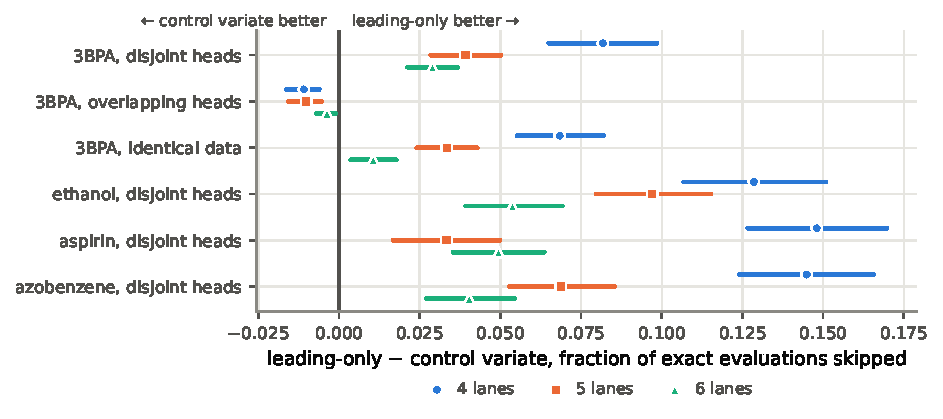
\includegraphics[width=\linewidth]{figures/fig2_gate_forest.pdf}
\caption{\textbf{Randomisation does not earn its backward passes.} Difference
in the fraction of exact evaluations skipped between the deterministic
leading-subspace estimator and the randomised low-rank sketch with control
variate, at three matched numbers of backward passes, with 95\% paired
block-bootstrap intervals. Positive means the deterministic estimator skips
more. The deterministic estimator wins significantly on $\fsLOBeatsCV$ of
$\fsLOSystems$ systems at every budget; the single exception is 3BPA with
overlapping heads, in a regime where both estimators already skip almost every
exact evaluation.}
\label{fig:gate}
\end{figure}

\subsubsection{A deterministic subspace beats a randomised sketch at equal cost}

Two estimators of the global score are compared at an equal number of backward
passes. The randomised low-rank sketch with control variate evaluates $r_0$
leading directions of the centred head space exactly and estimates the
remainder with random probe directions. This is the split that
\citet{meyer2021hutchpp} show to be optimal for estimating the value of a trace.
The deterministic leading-subspace estimator spends every backward pass on
exact leading eigendirections of the design-set head-space Gram matrix and
discards the remainder entirely. At every number of backward passes tested, the
deterministic estimator skips more on $\fsLOBeatsCV$ of $\fsLOSystems$ systems,
significantly under paired block-bootstrap intervals, and has no probe-seed
variance by construction (Figure~\ref{fig:gate}). The one exception is 3BPA with
overlapping heads, where the randomised sketch wins by a margin of no practical
consequence in a regime where both estimators already skip almost every exact
evaluation.

The mechanism is specific to calibrated screening rules. The constant
$c_\alpha$ is fitted to the ratio of the exact score to the cheap estimate, so
a systematic bias in the estimate is absorbed exactly. Only the variance of the
estimate costs skip fraction, because variance widens the ratio distribution
and pushes the calibrated constant up. The deterministic estimator is biased
low by construction and pays nothing for that bias. The randomised sketch is
unbiased but carries sampling variance, and the head-space spectrum of these
committees is concentrated: the stable rank of the centred head-space Gram
matrix is $\fsStableRankLo$--$\fsStableRankHi$ of a possible $r=M-1=7$, so a
random projection is being asked to resolve exactly what concentration makes
hard. The practical consequence is that the method gets simpler. At a fixed
number of backward passes, spend every pass on exact leading directions.

\begin{figure}[t]
\centering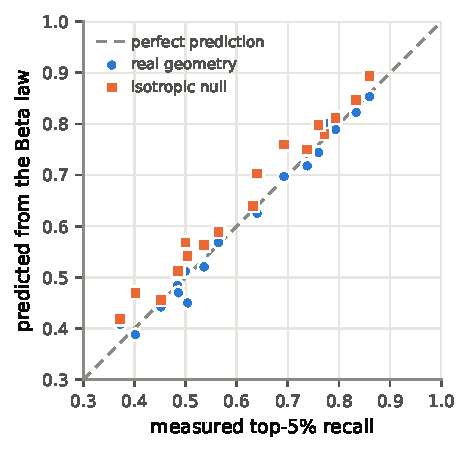
\includegraphics[width=0.52\linewidth]{figures/fig5_beta_law.pdf}
\caption{\textbf{A finite-sample law predicts the negative result with no
adjustable parameters.} Predicted against measured top-5\% recall for six
systems at three sketch sizes. Using the real head-space geometry gives a mean
absolute error of $\fsBetaMAE$; the isotropic null is both worse and
systematically optimistic, which is why coupling between coordinates cannot be
neglected.}
\label{fig:beta}
\end{figure}

\subsubsection{The failure of small randomised sketches is predictable}

For a sketch of $K$ uniformly random orthonormal (Haar) directions out of the
$r$ centred head-space directions, the ratio of estimated to true
per-coordinate variance is distributed exactly as
$\hat{v}_d/v_d \sim (r/K)\,\mathrm{Beta}(K/2,(r-K)/2)$. Injecting precisely
this noise into the exact variances and recomputing the top-5\% recall
reproduces the measured recall across six systems and three sketch sizes to a
mean absolute error of $\fsBetaMAE$, with no adjustable parameters
(Figure~\ref{fig:beta}). Two points follow. A common multiplicative bias cannot
change a rank statistic, so the damage is estimator variance, not bias. And the
coordinate directions cannot be treated as isotropic: using the real head-space
geometry roughly halves the prediction error relative to an isotropic null, so
coupling between coordinates matters.

A Chernoff bound makes the result structural rather than incidental. Uniform
accuracy of every per-coordinate variance to within a relative error of
$\varepsilon=0.1$ requires $K$ of order $10^{3}$--$10^{4}$ random directions,
against the $K\le r=7$ that a committee of eight heads can provide. The gap is
two to three orders of magnitude, so no tuning recovers the max-component rule
from a small random sketch.

\subsection{Committee size, and independently trained committees}
\label{sec:committees_results}

\subsubsection{Committee size}

Does any of the above need eight heads? We enumerated every subcommittee of
every size $m=2,\dots,8$ of each eight-head committee, $247$ subcommittees per
system across $20$ combinations of system and test regime, and measured the
error-ranking quality of each subcommittee relative to the full committee.
Positives are fixed by the full committee's reference error, so the question is
whether a smaller committee still finds the same high-error structures.
Halving the committee to $m=4$ retains $\fsMFourRetained$ of the full
committee's AUROC on average. The worst individual four-member subcommittee,
however, retains only $\fsMFourWorstSubset$, and the worst two-member
subcommittee retains $\fsMTwoWorstSubset$. Committee size therefore buys
insurance rather than accuracy: between four and eight heads the mean moves
little while the floor moves a great deal. A committee also does not become
calibrated in magnitude by growing. The overconfidence ratio defined below
improves only modestly from two heads to eight and stays far above one, so
magnitude calibration is a property of the construction rather than of the
number of heads.

\subsubsection{Independently trained committees}

The heads of a shared-trunk committee share almost all of their parameters. To
test which conclusions depend on that sharing, we evaluated independently
trained committees: eight full MACE models of the same architecture trained
from different random seeds, the construction \citet{beck2025committee} call a
naive committee and that is called a deep ensemble
elsewhere~\citep{lakshminarayanan2017simple}. Each independently trained
committee is matched to a shared-trunk committee on architecture, training data
and evaluation frames, so the construction is the only variable. The four pairs
are 3BPA with identical training data for every member (matched to the
identical-data heads), 3BPA with a different random 80\% of the training data
per member (matched to the overlapping heads), and liquid water on classical
molecular-dynamics frames and on path-integral frames (both matched to the
overlapping heads).

The global-score recommendation of Section~\ref{sec:fixedsize} holds for the
independently trained committees as well, so the recommendation is a property
of committees rather than of the multi-head architecture. The independently
trained committees are also far better calibrated in magnitude. We measure
magnitude calibration with the overconfidence ratio: the root-mean-square error
of the committee-mean force divided by the median per-atom committee standard
deviation. A ratio of one means the committee's spread matches its error, and a
larger ratio means the committee understates its error. On the four matched
pairs, with the independently trained committee quoted first, the ratio is
$\fsOverconfNaiveSame\times$ against $\fsOverconfSharedSame\times$ for 3BPA
with identical data, $\fsOverconfNaiveResampled\times$ against
$\fsOverconfSharedResampled\times$ for 3BPA with resampled data,
$\fsOverconfNaiveWaterMD\times$ against $\fsOverconfSharedWaterMD\times$ for
water on classical frames, and $\fsOverconfNaiveWaterPIMD\times$ against
$\fsOverconfSharedWaterPIMD\times$ for water on path-integral frames. Neither
construction is calibrated, but the two are not in the same league, and the gap
is widest where the heads share the most, on identical training data. The
independently trained committees are also more accurate on every matched pair
(Table~\ref{tab:accuracy}), so the shared-trunk construction trades accuracy
and calibration for the cost of a single trunk. The standardised-error view of
the same comparison is in Figure~\ref{fig:calibration}.

The acceleration does not transfer, and we state this as a derivation rather
than a measurement. With no shared trunk, the product $Fw$ of the per-head force
matrix with a head-space direction needs all $M$ columns of $F$, which is $M$
separate forward and backward passes. No sketch of the head space can be
cheaper than the exact quantity the sketch approximates. Of five predictions
pre-registered for this experiment, $\fsNaivePassed$ were confirmed. One
failure concerns the head-space spectrum under distribution shift and is
described in the Discussion; the other is the water result described next.

\subsection{Condensed phase and distribution shift}
\label{sec:water}

Bulk liquid water ($N=192$ atoms, periodic, $3N=576$ coordinates) tests the
molecular findings in the condensed phase. Two test sets at the same temperature,
one from classical molecular dynamics (MD) and one from path-integral molecular
dynamics (PIMD), give a distribution shift in which only quantum nuclear effects
differ. All water committees were trained on classical frames.

On the classical frames the error-ranking quality of the committee is the
weakest in this study, and the margin of the committee over the predicted force
norm is not significant. On the PIMD frames the shared-trunk committee's
error-ranking quality is the strongest in this study. One caveat must survive
contact with the reader. The strong PIMD result is substantially a symptom of
this model family failing badly there. The matched independently trained
committee is $\fsNaiveAccuracyRatio\times$ more accurate on the PIMD frames,
and once that accuracy is restored the committee's error-ranking quality
collapses to a level close to the classical frames, while the zero-cost force
norm retains most of the apparent skill of the shared-trunk committee. In other
words, where the shared-trunk model fails, the failure is dominated by a single
mode correlated with force magnitude, and a zero-cost baseline already detects
that mode. Any claim about committee uncertainty under distribution shift must
therefore be quoted beside the zero-cost baseline and beside the accuracy gap
(Table~\ref{tab:accuracy}), or the claim flatters the committee.

Distribution shift also degrades magnitude calibration more than it changes
ranking. For the shared-trunk water committee the overconfidence ratio rises
from $\fsOverconfSharedWaterMD\times$ on classical frames to
$\fsOverconfSharedWaterPIMD\times$ on PIMD frames, so the committee
under-responds to the shift by a wide margin. For a split-conformal screening
rule this is exactly the exchangeability violation the coverage guarantee
excludes: a constant calibrated on classical frames and deployed on PIMD frames
is fitted to a ratio distribution that has moved. The calibration constant must
be refitted per regime.

Finally, the ordering of the three scores is less clear-cut on water than on
the molecules. The global score keeps its advantage on the bulk-error targets
and is roughly tied with the max-component score on the maximum-based targets,
and on the PIMD frames the max-component score is ahead at every committee
size. The evidence for the global score is therefore strong on small molecules
and neutral on condensed-phase water, not universal.

% PASS2: 3.6 materials pool (in-distribution, filtered, out-of-distribution) goes here

% DRAFT: the subsection below covers only the parts of the materials-pool
% analysis whose numbers already exist. Pass 2 adds the filtered re-analysis and
% the OMat24 out-of-distribution scan (tab:ood) and may fold this draft into 3.6.
\subsection{Materials pool: in-distribution results}
\label{sec:materials_id}

The setting the screening rule is intended for is a foundation model carrying
committee readouts on a frozen trunk. We use the MACE-MP-0b medium
model~\citep{batatia2023foundation}, which is built on the MACE
architecture~\citep{batatia2022mace}, with the trunk frozen and eight disjoint
readout heads fine-tuned on a published query-by-committee selection of MPtraj
structures (Methods). The candidate pool is the complement of that selection:
$\fsMPtrajN$ periodic structures from MPtraj~\citep{deng2023chgnet} spanning 89
elements and 1--444 atoms, none of which the heads were fitted on. Two limits
of this experiment must be stated plainly, because the submitted version of
this paper did not state them. First, the MACE-MP-0b trunk was itself
pretrained on MPtraj. The pool is therefore in-distribution for the trunk and
out-of-sample only for the readout heads, and every number in this subsection
is an in-distribution number. Second, MPtraj contains many frames at or near
relaxed geometries, where the reference forces are close to zero. On such
frames a small predicted force norm and a small force error coincide for a
trivial reason, which favours the force-norm baseline discussed below. Two
further analyses answer these limits. A filtered re-analysis removes
near-equilibrium frames and single-atom cells and reports AUROC within
reference-force deciles; the result is \fsTODO{filtered-pool AUROC of the force
norm and of the committee scores, and the within-decile AUROC}. An
out-of-distribution scan on OMat24~\citep{barrosoluque2024omat24}, a dataset
that post-dates the trunk's training data, is reported in
Table~\ref{tab:ood}. Of the five predictions pre-registered for the
in-distribution scan, two were confirmed.

\subsubsection{Error ranking transfers to the materials pool}

Exact committee disagreement reaches AUROC $\fsMPtrajGlobal$ on this pool
against a random null of $\fsMPtrajRandom$. Committee force uncertainty is
therefore not an artefact of small organic molecules, and the random null at
chance is the check that the pipeline is sound at this scale.

\begin{figure}[t]
\centering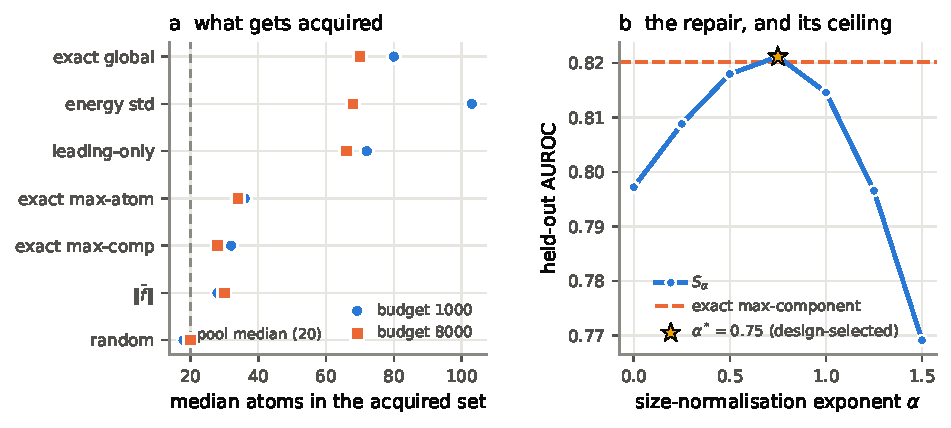
\includegraphics[width=\linewidth]{figures/fig3_extensivity.pdf}
\caption{\textbf{The global score is extensive, and size normalisation restores
parity rather than superiority.} (a) Median atom count of the structures
selected from the MPtraj pool by each score. The global score, and the two
quantities that inherit its sum over coordinates, select far larger structures
than the pool median; the max-component and max-atom scores and the predicted
force norm do not. (b) Held-out AUROC of the normalised score
$S_\alpha=(\sum_d v_d)/(3N)^\alpha$ against the exponent $\alpha$, with the
exponent $\alpha^*$ chosen on the design split marked by a star. The curve
peaks near the level of the max-component score, not above it.}
\label{fig:extensivity}
\end{figure}

\subsubsection{Extensivity, and why the global score reverses}

The global score sums $v_d$ over $3N$ coordinates, so the score grows with
system size whether or not the model is uncertain. Scores that sum over atoms
are known to carry this size dependence, which is why ensemble disagreement is
sometimes normalised by a power of the atom
count~\citep{smith2018less,kellner2024shallow,lortaraprasert2026size}. On the
MPtraj pool, selecting by the global score returns structures whose median atom
count is $\fsMPtrajExtensivity\times$ that of the max-component selection, and
the ordering of Section~\ref{sec:fixedsize} reverses on all four error targets
(Figure~\ref{fig:extensivity}a, Table~\ref{tab:mptraj}). Every system in
Section~\ref{sec:fixedsize} has one atom count, where an extensive and an
intensive score differ by a constant and this size bias cannot appear. The
fixed-size recommendation was never wrong where it was measured; it was
measured only where it could not fail.

The repair is a size normalisation, $S_\alpha=(\sum_d v_d)/(3N)^\alpha$, with
$\alpha$ chosen on a design split and every reported number taken from the
disjoint remainder of the pool. The selected $\alpha=\fsAlphaStar$ raises the
held-out AUROC from $\fsNormAurocZero$ to $\fsNormAurocStar$
(Figure~\ref{fig:extensivity}b). At fixed $N$ the normalisation changes nothing,
exactly, so it can be adopted everywhere at no cost. We report the outcome
precisely: across the four error targets the normalised score achieves
$\fsNormWins$ significant wins, one tie and $\fsNormLosses$ significant loss
against the max-component score. Normalisation restores parity, not
superiority, and the best exact committee score on this pool is the max-atom
score (Table~\ref{tab:mptraj}). The exponent $\alpha$ depends on the pool and
on the error target rather than being universal: an intensive target such as a
root-mean-square error favours a larger exponent than a maximum-based target.

\begin{table}[t]
\centering
\caption{\textbf{On the in-distribution materials pool a zero-cost baseline
outranks every committee score.} AUROC on $\fsMPtrajN$ MPtraj structures under a
frozen foundation-model trunk, for four error targets. The row labelled
$\|\bar{f}\|$ is the predicted force norm, a by-product of the forward pass; the
row labelled energy std is the spread of the head energies; the row labelled
leading-only is the deterministic leading-subspace estimator at five backward
passes. The last two columns are post-hoc diagnostics: AUROC recomputed within
atom-count quartiles and within force-magnitude quintiles, so that neither the
size bias nor force magnitude itself can explain the ordering. The predicted
force norm is in bold because it costs nothing.}
\label{tab:mptraj}
\small
\begin{tabular}{lcccccc}
\toprule
& \multicolumn{4}{c}{AUROC by error score} & \multicolumn{2}{c}{stratified (post hoc)}\\
\cmidrule(lr){2-5}\cmidrule(lr){6-7}
signal & $e_{\max}$ & $e_{\mathrm{rmse}}$ & $e_{\max\mathrm{c}}$ & $e_{q95}$ & by size & by force \\
\midrule
exact max-atom & 0.836 & 0.819 & 0.824 & 0.806 & -- & 0.649 \\
exact max-component & 0.821 & 0.808 & 0.822 & 0.805 & 0.798 & 0.656 \\
exact global & 0.798 & 0.769 & 0.793 & 0.759 & 0.794 & 0.632 \\
leading-only, 5 lanes & 0.791 & 0.763 & 0.786 & 0.753 & 0.779 & 0.626 \\
$\|\bar{f}\|$ \emph{(zero cost)} & \textbf{0.943} & \textbf{0.933} & \textbf{0.942} & \textbf{0.930} & \textbf{0.933} & \textbf{0.710} \\
energy std \emph{(zero cost)} & 0.481 & 0.447 & 0.483 & 0.450 & 0.394 & 0.511 \\
random null & 0.499 & 0.498 & 0.498 & 0.498 & -- & 0.499 \\
\bottomrule
\end{tabular}

\end{table}

\subsubsection{The zero-cost baseline wins here, and is not complemented}

The predicted force norm reaches AUROC $\fsMPtrajFree$ against the committee's
$\fsMPtrajGlobal$: a quantity already computed in the forward pass outranks
eight backward passes (Table~\ref{tab:mptraj}). The advantage survives
stratification by atom count. Within force-magnitude quintiles the committee
still beats chance, so the committee does carry information beyond force
magnitude; the zero-cost baseline is simply at least as good. The head-energy
spread, by contrast, is at or below chance on this pool.

We do not present this as a surprising property of committees. Force errors
tend to grow with force magnitude, so the predicted force norm is a strong
baseline wherever the largest forces are also where the model is most wrong,
and the near-equilibrium frames in MPtraj make the correspondence especially
tight. The claim we make is narrower: committee methods must be scored against
this baseline rather than against a random null, and the filtered and
out-of-distribution analyses (\fsTODO{filtered-pool and OMat24 force-norm versus
committee AUROC}) together with the active-learning round of
Table~\ref{tab:al} bound where the baseline's advantage holds.

Because the force norm is already available, the decision a practitioner faces
is not ``committee or baseline'' but ``baseline, or baseline plus eight
backward passes''. Nested logistic models fitted on a design split and scored
on held-out data give AUROC $\fsCompFree$ for the force norm alone and
$\fsCompBoth$ with the committee added, a marginal gain of $\fsCompMarginal$
that is not significant. On the fixed-composition systems of
Sections~\ref{sec:fixedsize} to~\ref{sec:water} the same comparison gives
significant gains on $\fsCompFixedSig$ of $\fsCompFixedN$ systems, spanning
$\fsCompFixedLo$--$\fsCompFixedHi$. The committee is redundant here, not in
general, and the discriminating variable is how close the zero-cost baseline
already is to saturation.

\subsubsection{The selection-overlap bound is unavailable}

One can hope to bound the downstream active-learning difference without
retraining by showing that the screening rule selects nearly the same set as
the exact statistic. On this pool it does not. The Jaccard overlap between the
selection of the deterministic leading-subspace estimator and the selection of
the exact global score is $\fsMPtrajJaccard$ at a realistic selection rate,
short of the pre-registered threshold. Overlap statistics must always be
reported with their selection rate, because any two rankings agree when a large
fraction of the pool is taken. Whether the difference in selected structures
costs anything after retraining is the question the active-learning round of
Table~\ref{tab:al} addresses directly.

% PASS2: 3.7 active-learning round goes here

\begin{figure}[t]
\centering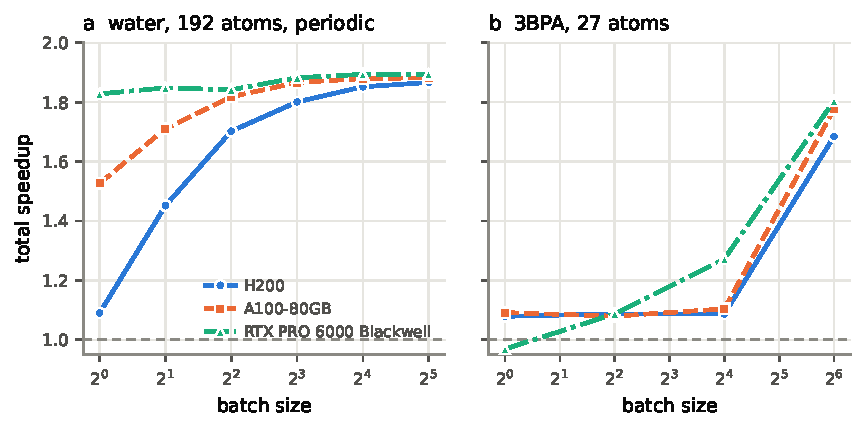
\includegraphics[width=\linewidth]{figures/fig4_speedup.pdf}
\caption{\textbf{Reducing the number of backward passes saves time once the
backward pass is compute-bound, and the batch size at which that happens rises
with machine speed.} Total speedup of the committee force evaluation against
batch size for (a) water and (b) 3BPA, measured with both systems in a single
exclusive job per device. Water converges to
$\fsWaterSpeedupBSixteen\times$--$\fsWaterSpeedupBSixteenBlk\times$ by $B=16$ on
all three architectures; 3BPA stays near $\fsThreeBPASpeedupBSixteen\times$
except on Blackwell. The H200 is the fastest machine and is still launch-bound
at $B=1$.}
\label{fig:speedup}
\end{figure}

\begin{table}[t]
\centering
\caption{\textbf{Pre-registered timing predictions, scored per device on matched
pairs.} Water and 3BPA measured in one exclusive job per device at identical
settings. v2 is the frozen pre-registered protocol; v3 is a post-hoc repair that
derives its reference from the matched 3BPA run rather than from a fixed
constant, and the repair changes the score only on Blackwell. P1 and P2, the
predictions that carry the speedup claim, pass on every device.}
\label{tab:pairs}
\small
\begin{tabular}{lccccccc}
\toprule
& \multicolumn{2}{c}{verdict} & \multicolumn{4}{c}{pre-registered predictions} & speedup \\
\cmidrule(lr){2-3}\cmidrule(lr){4-7}\cmidrule(lr){8-8}
device & v2 & v3 & P1 & P2 & P3 & P4 & water, $B{=}16$ \\
\midrule
H200 & \textbf{4/4} & 4/4 & \checkmark & \checkmark & \checkmark & \checkmark & 1.852$\times$ \\
A100-SXM4-80GB & \textbf{3/4} & 3/4 & \checkmark & \checkmark & $\times$ & \checkmark & 1.880$\times$ \\
RTX PRO 6000 Blackwell & \textbf{2/4} & 3/4 & \checkmark & \checkmark & $\times$ & $\times$ & 1.894$\times$ \\
\bottomrule
\end{tabular}

\end{table}

\subsection{Wall clock}
\label{sec:wallclock}

Reducing the number of backward passes saves time only once the backward pass
is compute-bound rather than launch-bound, and the controlling variable is the
total number of graph edges in the batch, not the number of structures. The
comparison is an exact committee evaluation with eight backward passes against
an estimate with four. Measuring both systems in a single exclusive job at
identical settings, water reaches $\fsWaterSpeedupBOne\times$ at batch size
$B=1$, rising to $\fsWaterSpeedupBSixteen\times$ at $B=16$ on an A100,
$\fsWaterSpeedupBSixteenHTwo\times$ on an H200 and
$\fsWaterSpeedupBSixteenBlk\times$ on an RTX PRO 6000 Blackwell, three GPU
generations agreeing to $\fsWaterSpeedupSpread$\%. 3BPA in the same job
reaches $\fsThreeBPASpeedupBSixteen\times$ at $B=16$ on the A100
(Figure~\ref{fig:speedup}, Table~\ref{tab:pairs}). Because the threshold is a
property of the machine as well as of the system, the batch size at which the
saving begins increases with how fast the GPU is; the H200 is the fastest
machine measured and is still launch-bound at $B=1$.

Acceleration is deliberately not the headline. The count of avoided exact
evaluations in Section~\ref{sec:screeningresults} does not depend on hardware
and survives every timing outcome.
